\documentclass[10pt]{article}
\usepackage[fontsize=10pt]{fontsize}

\usepackage[margin=0.5in]{geometry} 
\usepackage{amsmath,amsthm,amssymb, graphicx, multicol, array, txfonts}
\usepackage{bbm}
\usepackage{hyperref}
\hypersetup{
    colorlinks=true,
    linkcolor=blue,
    filecolor=magenta,      
    urlcolor=cyan,
    pdftitle={Overleaf Example},
    pdfpagemode=FullScreen,
    }

\urlstyle{same}


\newcommand{\N}{\mathbb{N}}
\newcommand{\Z}{\mathbb{Z}}
\setcounter{secnumdepth}{0}
\setlength\parindent{0pt}

 
\newenvironment{problem}[2][Problem]{\begin{trivlist}
\item[\hskip \labelsep {\bfseries #1}\hskip \labelsep {\bfseries #2.}]}{\end{trivlist}}

\newenvironment{prelim}[2][Preliminaries]{\begin{trivlist}
\item[\hskip \labelsep {\bfseries #1}\hskip \labelsep {\bfseries #2}]}{\end{trivlist}}
    
\begin{document}
 
\title{6.S091 Problem Set 2}
\author{Suyeol Yun\\
6.S091: Causality}
\maketitle
 
\section{Problem 1}
\subsection{Plotting Regression Residuals}
\subsection{(a)} $\hat{\beta}_{12} = 2.0032613606359835$
\subsection{(b)} $\hat{\beta}_{21} = 0.4853818665988653$

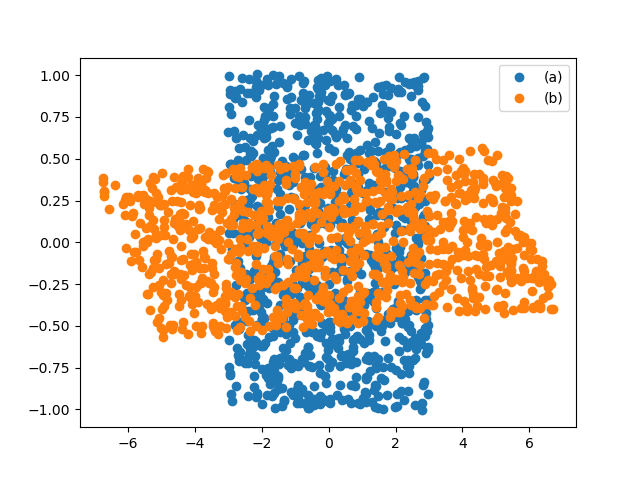
\includegraphics{images/problem1.png}

\subsection{Causal Direction Inference}

\subsection{(c)}
The plot explains the relationship between $\varepsilon_1$ and $\varepsilon_2$. Since $\varepsilon_1 \Perp \varepsilon_2$, we have to choose the SCM which shows such independence. Therefore, the data is more likely to be generated from SCM $M^a$.


\end{document}
